\chapter{Stato dell'Arte del 3D Gaussian Splatting}
\label{chap:arte}

\section{Fondamenti di rendering 3D}

Prima di analizzare le tecniche di rappresentazione 3D e il Gaussian Splatting, è necessario introdurre alcuni concetti fondamentali del rendering tridimensionale che costituiscono la base teorica per la comprensione degli argomenti trattati in questo lavoro.

\subsection{Pipeline di rendering}

Il rendering 3D è il processo di generazione di immagini bidimensionali a partire da scene tridimensionali. La pipeline di rendering tradizionale può essere suddivisa in fasi principali:

\begin{enumerate}
    \item \textbf{Trasformazione geometrica}: conversione delle coordinate degli oggetti 3D dallo spazio mondiale al sistema di coordinate della camera
    \item \textbf{Proiezione}: mappatura dei punti 3D sul piano immagine 2D attraverso la camera virtuale
    \item \textbf{Rasterizzazione}: conversione delle primitive geometriche in pixel discreti
    \item \textbf{Shading}: calcolo del colore finale di ogni pixel considerando illuminazione e materiali
\end{enumerate}

\newpage  % ✨ AGGIUNGI QUESTA RIGA
\subsection{Tecniche di rendering}

Esistono due paradigmi principali per il rendering 3D:

\begin{itemize}
	\item \textbf{Rasterizzazione}: Tecnica che processa le primitive geometriche (triangoli, punti) \textbf{proiettandole} direttamente sul piano immagine. È altamente efficiente e ottimizzata per hardware GPU, permettendo rendering real-time. Tuttavia, gestisce con difficoltà effetti ottici complessi come riflessioni accurate e trasparenze multiple.

\item \textbf{Ray tracing}: Metodo che simula il percorso fisico della luce \textbf{lanciando} raggi virtuali dalla camera attraverso ogni pixel dell'immagine. Offre realismo superiore nella gestione di riflessioni, rifrazioni e ombre, ma richiede maggiori risorse computazionali.
\end{itemize}

\begin{figure}[htbp]
	\centering
	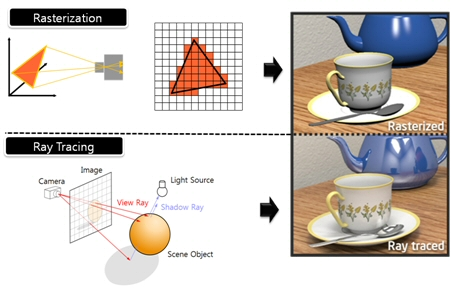
\includegraphics[width=1\textwidth]{images/rasterization_vs_ray_tracing.jpg}
	\caption{Rasterizzazione vs Ray tracing}
	Fonte: \cite{rasterization_vs_ray_tracing}
\end{figure}

\newpage
\subsection{Proiezione e volume di visibilità}

La trasformazione da spazio 3D a immagine 2D avviene attraverso il concetto di \textbf{view frustum}, che definisce precisamente quale porzione dello spazio 3D sarà visibile nell'immagine finale.

\subsubsection{Il view frustum}

Il view frustum è un volume tronco-piramidale con vertice nel punto di osservazione della camera (eye point). È delimitato da sei piani:

\begin{itemize}
    \item \textbf{Near plane}: Il piano più vicino alla camera, definisce la distanza minima di rendering
    \item \textbf{Far plane}: Il piano più lontano, oltre il quale gli oggetti non vengono renderizzati
    \item \textbf{Left/Right planes}: Delimitano l'estensione orizzontale del campo visivo
    \item \textbf{Top/Bottom planes}: Definiscono l'estensione verticale del campo visivo
\end{itemize}

Il frustum è caratterizzato da parametri chiave: il \textbf{field of view} (FOV) che determina l'ampiezza angolare della visione, l'\textbf{aspect ratio} che definisce il rapporto larghezza/altezza dell'immagine, e le distanze \textbf{near} e \textbf{far} che stabiliscono l'intervallo di profondità renderizzabile.

\begin{figure}[htbp]
    \centering
    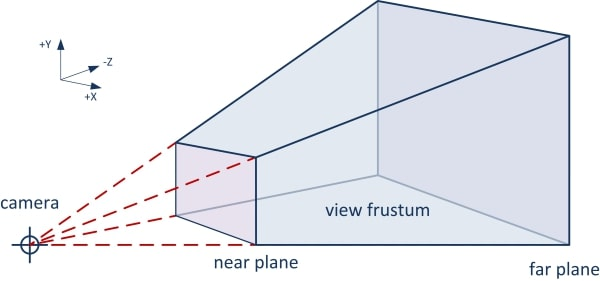
\includegraphics[width=0.9\textwidth]{images/view_frustum.jpg}
    \caption{Rappresentazione del view frustum}
    Fonte: \cite{view_frustum}
\end{figure}

\subsubsection{Tipi di proiezione}

I due tipi principali di proiezione determinano forme diverse del volume di visibilità:

\begin{itemize}
 \item \textbf{Proiezione parallela (o ortografica)}  utilizza raggi paralleli per proiettare gli oggetti sul piano immagine, mantenendo le dimensioni relative costanti indipendentemente dalla distanza. In questo caso, il volume di visibilità non è più un frustum ma diventa un \textbf{parallelepipedo retto} con pareti parallele, poiché non c'è convergenza dei raggi verso un punto di osservazione. Sebbene sia utile per applicazioni CAD e disegno tecnico dove è necessario preservare proporzioni e misure esatte, non è adatta per il rendering 3D realistico poiché non simula la percezione visiva umana.
 \item \textbf{Proiezione prospettica} mantiene invece la forma tronco-piramidale del view frustum, facendo convergere i raggi di proiezione verso il punto di osservazione della camera. Gli oggetti più distanti appaiono più piccoli a causa della convergenza geometrica del frustum, creando un senso naturale di profondità e realismo visivo.
\end{itemize}



\begin{figure}[htbp]
    \centering
    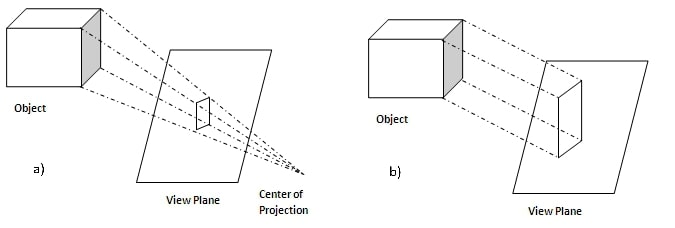
\includegraphics[width=0.8\textwidth]{images/perspective_vs_parallel.jpg}
    \caption{Tipi di proiezione: a) proiezione prospettica b) proiezione parallela}
    Fonte: \cite{projection_types}
\end{figure}
\newpage
 Le rispettive \textbf{matrici di proiezione}, costruite a partire dai parametri del frustum (FOV, aspect ratio, near/far), trasformano le coordinate 3D in coordinate di clip normalizzate, permettendo contemporaneamente la corretta proiezione e l'eliminazione automatica (culling) di geometrie esterne al volume visibile.

\begin{equation}
	P_{ortho} = \begin{pmatrix}
		\frac{2}{r-l} & 0 & 0 & -\frac{r+l}{r-l} \\
		0 & \frac{2}{t-b} & 0 & -\frac{t+b}{t-b} \\
		0 & 0 & -\frac{2}{f-n} & -\frac{f+n}{f-n} \\
		0 & 0 & 0 & 1
	\end{pmatrix}
\end{equation}
\begin{center}
	\textit{Matrice di proiezione ortografica}
\end{center}

\begin{equation}
P_{persp} = \begin{pmatrix}
\frac{2n}{r-l} & 0 & \frac{r+l}{r-l} & 0 \\
0 & \frac{2n}{t-b} & \frac{t+b}{t-b} & 0 \\
0 & 0 & -\frac{f+n}{f-n} & -\frac{2fn}{f-n} \\
0 & 0 & -1 & 0
\end{pmatrix}
\end{equation}
\begin{center}
	\textit{Matrice di proiezione prospettica}
\end{center}

dove $n$ = near plane, $f$ = far plane, $l$ = left, $r$ = right, $t$ = top, $b$ = bottom.
\newline
\noindent La differenza fondamentale risiede nella terza riga: la proiezione prospettica introduce il fattore $-1$ nell'elemento $(4,3)$ che causa la divisione prospettica (trasformazione da coordinate omogenee), mentre la proiezione ortografica mantiene $w = 1$, preservando le proporzioni.

\subsection{Rasterizzazione}

La \textbf{rasterizzazione} è il processo di conversione delle primitive geometriche continue (triangoli, linee, punti) in pixel discreti su una griglia 2D. Rappresenta la fase finale della pipeline di rendering dove le forme geometriche vengono "disegnate" nell'immagine.

Il processo avviene attraverso questi passaggi:

\begin{itemize}
    \item \textbf{Scan conversion}: Determinazione di quali pixel dell'immagine sono coperti da ogni primitiva geometrica
    \item \textbf{Interpolazione}: Calcolo dei valori degli attributi (colore, coordinate texture, normali) per ogni pixel attraverso interpolazione baricentrica nei triangoli
    \item \textbf{Z-buffering}: Gestione della visibilità tramite buffer di profondità per determinare quale superficie è più vicina alla camera
    \item \textbf{Shading}: Applicazione di modelli di illuminazione per calcolare il colore finale di ogni pixel
\end{itemize}

\begin{figure}[htbp]
    \centering
    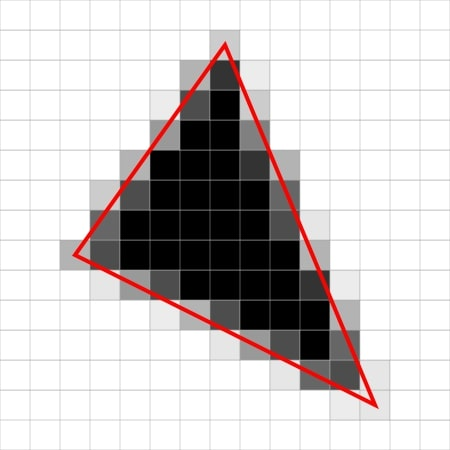
\includegraphics[width=0.5\textwidth]{images/rasterization.jpg}
    \caption{Triangolo 3D rappresentato su uno schermo}
    Fonte: \cite{rasterization}
\end{figure}

\subsection{Considerazioni per GPU moderne}
La rasterizzazione è altamente ottimizzata per le GPU moderne grazie alla sua struttura adatta alle pipeline grafiche tradizionali: processa primitive geometriche in sequenza attraverso stadi fissi. Questo la rende ideale per applicazioni real-time.

\noindent Il ray tracing, pur essendo anch'esso intrinsecamente parallelo (ogni raggio può essere tracciato indipendentemente), richiede strutture dati complesse per l'accelerazione spaziale e accessi di memoria meno prevedibili, risultando tradizionalmente più costoso computazionalmente. Tuttavia, le GPU moderne con unità RT (Ray Tracing) dedicate stanno rendendo il ray tracing sempre più competitivo anche per applicazioni real-time.
\noindent Le GPU moderne sono ottimizzate per parallelismo massivo e throughput elevato. 
Tra le caratteristiche e gli aspetti piu importanti abbiamo:

\begin{itemize}
    \item \textbf{Parallelizzazione}: Migliaia di thread processano simultaneamente diversi pixel o primitive
    \item \textbf{Memory bandwidth}: La velocità di accesso alla memoria è spesso il fattore limitante
    \item \textbf{Coerenza spaziale}: Algoritmi che sfruttano la località spaziale dei dati ottengono prestazioni superiori
\end{itemize}

\noindent Questi principi fondamentali influenzano profondamente la progettazione di tecniche moderne come il 3D Gaussian Splatting, che combina l'efficienza della rasterizzazione con la flessibilità di rappresentazioni alternative alle mesh tradizionali.
\section{Panorama delle rappresentazioni 3D}
\label{sec:panoramica}

\subsubsection{Tecniche tradizionali}
Le rappresentazioni 3D tradizionali si basano principalmente su mesh poligonali e point clouds, che differiscono fondamentalmente nella loro organizzazione dei dati.
\newline\newline
Le \textbf{mesh poligonali} rappresentano dati strutturati: utilizzano triangoli interconnessi per definire superfici continue, dove ogni vertice è connesso ad altri vertici per formare spigoli, che a loro volta si collegano per creare facce triangolari. Questa struttura interconnessa garantisce rappresentazioni geometriche precise e compatibilità con le pipeline di rendering tradizionali, ma richiede maggiore complessità computazionale per la gestione delle connessioni. Inoltre, presentano limitazioni nella gestione di geometrie complesse come capelli, fumo o superfici trasparenti.
\newline\newline
Le \textbf{point clouds}, d'altra parte, rappresentano dati non strutturati: consistono in insiemi discreti di punti nello spazio 3D, ciascuno con posizione e colore associati, ma senza informazioni di connessione tra di essi. Questa caratteristica le rende più semplici da renderizzare dal punto di vista computazionale, poiché ogni punto può essere processato indipendentemente. Sebbene siano efficaci per la cattura di dati da sensori come LiDAR\footnote{Il \textit{LiDAR} (Light Detection and Ranging) è una tecnologia di telerilevamento che misura la distanza dagli oggetti usando impulsi laser. Viene comunemente impiegata per ottenere mappe 3D precise di ambienti, sia in ambito terrestre che aereo.}, soffrono di discontinuità visive e difficoltà nel rendering di superfici smooth.
\begin{figure}[htbp]
    \centering
    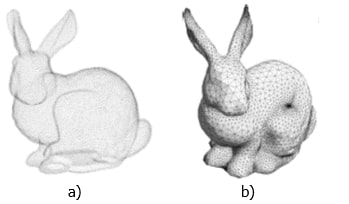
\includegraphics[width=0.9\textwidth]{images/rabbits.jpg}
    \caption{Esempi di modelli 3D: a) point cloud b) mesh poligonale}
    Fonte: \cite{researchgate_bunny}
\end{figure}
Le limitazioni delle rappresentazioni discrete appena citate hanno portato allo sviluppo di approcci volumetrici, che modellano lo spazio 3D come un continuum di proprietà ottiche piuttosto che attraverso elementi geometrici separati.

\subsection{Volume Rendering: verso rappresentazioni continue}

Le limitazioni delle mesh poligonali e dei point clouds hanno portato allo sviluppo di approcci alternativi basati su rappresentazioni volumetriche. Il volume rendering rappresenta un paradigma fondamentale che modella fenomeni difficili da rappresentare con primitive geometriche tradizionali.

\subsubsection{Principi fondamentali}

Come definito da \cite{ikits2004volume}, "Direct volume rendering methods generate images of a 3D volumetric data set without explicitly extracting geometric surfaces from the data". Questa tecnica utilizza un modello ottico per mappare i valori dei dati a proprietà ottiche come colore e opacità.

Il volume rendering assume che il volume sia composto da particelle che simultaneamente emettono e assorbono luce \cite{ikits2004volume}. Durante il rendering, le proprietà ottiche vengono accumulate lungo ogni raggio di vista per formare un'immagine dei dati. Ogni elemento di volume (voxel) corrisponde a una posizione nello spazio dei dati e ha uno o più valori associati.

Il processo di generazione dell'immagine avviene attraverso il campionamento del volume lungo tutti i raggi di vista e l'accumulo delle proprietà ottiche risultanti \cite{ikits2004volume}. Per il modello di emissione-assorbimento, il colore e l'opacità accumulati vengono calcolati iterativamente, ordinando i campioni lungo il raggio di vista.

\begin{figure}[htbp]
    \centering
    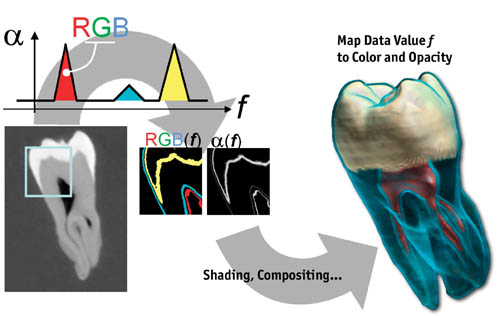
\includegraphics[width=0.9\textwidth]{images/volume_rendering_process.jpg}
    \caption{Il processo del volume rendering}
    Fonte: \cite{volume_rendering_process}
\end{figure}

\subsubsection{Fenomeni volumetrici}

Molti effetti visivi sono di natura volumetrica \cite{ikits2004volume}. Fluidi, nuvole, fuoco, fumo, nebbia e polvere sono difficili da modellare con primitive geometriche. I modelli volumetrici sono meglio adatti per creare tali effetti, poiché assumono che la luce venga emessa, assorbita e diffusa da un gran numero di particelle nel volume.

\subsubsection{Applicazioni scientifiche e ingegneristiche}

Oltre alla modellazione di fenomeni volumetrici, il volume rendering è essenziale per applicazioni scientifiche e ingegneristiche che richiedono la visualizzazione di dataset tridimensionali \cite{ikits2004volume}. Gli esempi includono:

\begin{itemize}
    \item \textbf{Imaging medico}: visualizzazione di dati acquisiti da dispositivi di imaging medicale
    \item \textbf{Simulazioni fluidodinamiche}: visualizzazione di risultati da simulazioni computazionali
    \item \textbf{Esplorazione scientifica}: analisi interattiva di dati volumetrici complessi
\end{itemize}

Gli utenti di applicazioni di volume rendering interattivo si affidano alle prestazioni degli acceleratori grafici moderni per un'esplorazione efficiente dei dati e la scoperta di caratteristiche.

\subsubsection{Limitazioni tecniche}

Il volume rendering presenta diverse sfide computazionali significative \cite{ikits2004volume}:

\begin{itemize}
    \item \textbf{Richieste hardware elevate}: necessita di computer molto potenti per ottenere risultati in tempo reale
    \item \textbf{Velocità di rendering limitata}: il processo è più lento rispetto al rendering di oggetti solidi tradizionali
    \item \textbf{Consumo di memoria}: i dati volumetrici richiedono grandi quantità di memoria per scene dettagliate
    \item \textbf{Complessità algoritmica}: gli algoritmi necessari sono matematicamente e computazionalmente complessi
\end{itemize}

\subsubsection{Evoluzione verso tecniche moderne}

Il volume rendering ha costituito la base teorica per lo sviluppo di tecniche moderne di \textbf{novel view synthesis}, cioè la generazione di immagini realistiche di una scena da angolazioni o posizioni di osservazione non presenti nel set originale di immagini. Le tecniche texture-based descritte da \cite{ikits2004volume} hanno dimostrato come sia possibile combinare facilmente algoritmi poligonali con volume rendering, richiedendo solo pochi pass di rendering e offrendo un alto livello di interattività senza sacrificare la qualità del rendering.
\newline
\newline
Questa flessibilità ha aperto la strada a rappresentazioni ibride che combinano i vantaggi del volume rendering con l'efficienza di primitive esplicite. Prima i Neural Radiance Fields (NeRF), poi il 3D Gaussian Splatting, possono essere visti come un'evoluzione naturale di questi concetti, mantenendo la capacità di rappresentare fenomeni volumetrici complessi.
\newline
\newline
L'eredità del volume rendering è particolarmente evidente nella gestione delle proprietà ottiche e nell'accumulo lungo i raggi di vista, principi che rimangono centrali nelle tecniche moderne di neural rendering e rappresentazioni gaussiane.

\subsubsection{Neural Radiance Fields (NeRF)}

L'evoluzione del volume rendering verso approcci basati su machine learning ha trovato la sua espressione più innovativa nei Neural Radiance Fields (NeRF), introdotti da \cite{mildenhall2020nerf}. Questa tecnica rappresenta un salto paradigmatico nella rappresentazione di scene 3D, utilizzando reti neurali per codificare implicitamente volumi continui attraverso funzioni differenziabili.

\begin{figure}[htbp]
	\centering
	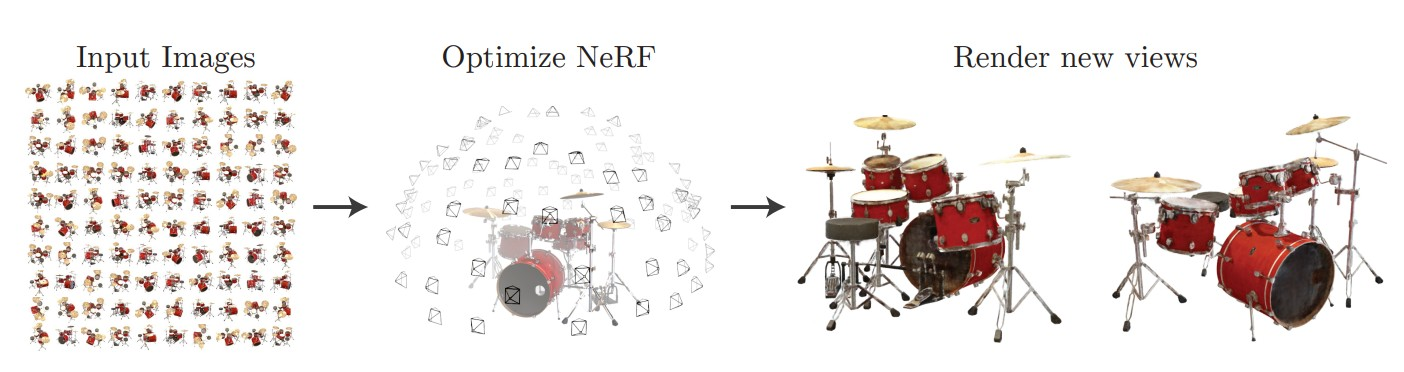
\includegraphics[width=0.9\textwidth]{images/5d_optimization.jpg}
	\caption{Ottimizzazione di una rappresentazione 5D continua}
	Fonte: \cite{5d_optimization}
\end{figure}

\paragraph{Rappresentazione 5D continua}
NeRF modella una scena statica come una funzione continua 5D che mappa coordinate spaziali 3D $(x, y, z)$ e direzioni di vista 2D $(\theta, \phi)$ a proprietà ottiche: densità volumetrica $\sigma$ e colore emesso dipendente dalla vista $(r, g, b)$. Questa rappresentazione viene approssimata attraverso una rete neurale Multi-Layer Perceptron (MLP)\footnote{Un \textit{Multi-Layer Perceptron} (MLP) è una rete neurale artificiale composta da più strati di neuroni completamente connessi. È in grado di apprendere relazioni non lineari tra input e output attraverso l'addestramento supervisionato.} completamente connessa $F_\Theta : (x, d) \rightarrow (c, \sigma)$, dove $\Theta$ rappresenta i pesi ottimizzabili della rete.

L'architettura impone vincoli di consistenza multi-vista: la densità volumetrica $\sigma$ dipende esclusivamente dalla posizione spaziale $x$, mentre il colore RGB $c$ può variare in funzione sia della posizione che della direzione di vista $d$. Questa separazione consente di rappresentare effetti non-Lambertiani\footnote{Gli \textit{effetti non-Lambertiani} sono fenomeni ottici in cui la luce riflessa da una superficie varia in base all’angolo di osservazione, come accade con i riflessi speculari, le superfici lucide o traslucide. Diversamente dai materiali Lambertiani, che riflettono la luce in modo uniforme, questi effetti dipendono dalla direzione della visuale.} come riflessi speculari e variazioni di colore dipendenti dall'angolo di osservazione.

\paragraph{Rendering volumetrico differenziabile}
Il processo di rendering utilizza principi classici del volume rendering per accumulare colore e opacità lungo raggi camera. Per un raggio $r(t) = o + td$ con limiti near e far $t_n$ e $t_f$, il colore atteso $C(r)$ viene calcolato attraverso l'integrale:

\begin{equation}
	C(r) = \int_{t_n}^{t_f} T(t)\sigma(r(t))c(r(t), d)dt
\end{equation}

dove $T(t) = \exp(-\int_{t_n}^{t} \sigma(r(s))ds)$ rappresenta la trasmittanza accumulata lungo il raggio. L'integrale viene approssimato numericamente attraverso campionamento stratificato, evitando le limitazioni di risoluzione delle griglie voxel discrete.

\paragraph{Innovazioni tecniche}
NeRF introduce due miglioramenti fondamentali per ottenere risultati di qualità elevata:

\begin{itemize}
\item \textbf{Positional Encoding}: Le coordinate di input vengono mappate in uno spazio dimensionale superiore utilizzando funzioni sinusoidali ad alta frequenza. Questo approccio, ispirato ai Transformer\footnote{I \textit{Transformer} sono un'architettura di rete neurale basata sull'attenzione, progettata per elaborare sequenze di dati (come testo o tempo) senza l'uso di strutture ricorrenti. Introdotti nel contesto del Natural Language Processing, usano il \textit{positional encoding} per incorporare informazioni sulla posizione degli elementi nella sequenza.}, consente alla rete di rappresentare dettagli ad alta frequenza che altrimenti verrebbero smussati dalla tendenza delle reti neurali verso funzioni a bassa frequenza.

\item \textbf{Campionamento gerarchico}: Il sistema utilizza due reti distinte ("coarse" e "fine") per allocare efficientemente i punti di campionamento. La rete coarse fornisce una distribuzione di probabilità che guida un campionamento più informato per la rete fine, concentrando le risorse computazionali nelle regioni più rilevanti del volume.
\end{itemize}

\paragraph{Vantaggi e limitazioni}
I Neural Radiance Fields hanno dimostrato capacità superiori nella sintesi di nuove viste rispetto ai metodi precedenti, particolarmente nella rappresentazione di scene complesse con geometrie intricate e materiali non-Lambertiani. La rappresentazione continua elimina gli artefatti di discretizzazione tipici delle griglie voxel, mentre i requisiti di memoria sono significativamente ridotti rispetto agli approcci volumetrici tradizionali.

Tuttavia, NeRF presenta limitazioni significative in termini di efficienza computazionale. Il training richiede tipicamente 1-2 giorni su GPU high-end per singole scene, mentre il rendering è computazionalmente intensivo, richiedendo centinaia di milioni di query alla rete per singola immagine. Questa inefficienza limita l'applicabilità in contesti real-time o interattivi.

\paragraph{Impatto e eredità}
NeRF ha stabilito i fondamenti teorici per una nuova generazione di tecniche di novel view synthesis, influenzando lo sviluppo di rappresentazioni ibride che combinano i vantaggi del rendering volumetrico con primitive più efficienti. I principi di rappresentazione continua, rendering differenziabile e ottimizzazione basata su immagini costituiscono l'eredità concettuale che ha ispirato successive innovazioni come il 3D Gaussian Splatting.
\section{Fondamenti teorici del Gaussian Splatting}
\subsection{Rappresentazione 3D basata su gaussiane}

Il 3D Gaussian Splatting introduce un paradigma innovativo per la rappresentazione di scene tridimensionali, utilizzando primitive gaussiane 3D come elementi fondamentali in alternativa alle tradizionali mesh poligonali o ai Neural Radiance Fields impliciti.

Mentre le metodologie consolidate si basano su mesh poligonali progettate da artisti 3D o su nuvole di punti generate tramite tecniche di fotogrammetria classica, il 3D Gaussian Splatting adotta un approccio radicalmente diverso. Il dataset di partenza consiste in foto o video acquisiti direttamente da oggetti o scene del mondo reale, oppure in scene sintetiche generate artificialmente tramite motori grafici o dataset simulati. Questi dati vengono successivamente elaborati attraverso algoritmi specializzati per generare una rappresentazione tridimensionale fotorealistica basata su primitive gaussiane.

Questa metodologia offre il vantaggio significativo di catturare scene complesse del mondo reale con un livello di fedeltà visiva superiore, preservando dettagli come riflessi accurati ed effetti anisotropi direzionali che risultano difficili da riprodurre con le tecniche tradizionali di computer grafica.

\paragraph{Il concetto di "Splats" nella computer grafica
}
Per comprendere meglio il concetto di primitiva gaussiana, è utile introdurre il termine "splats", una tecnica di computer grafica introdotta nel 2001 che ha trovato diverse applicazioni nel rendering 3D. Nel contesto del rendering di point cloud, gli splats hanno dimostrato la loro efficacia nel migliorare significativamente la qualità visiva delle rappresentazioni basate su punti.
Quando si renderizza una point cloud tradizionale, ogni punto viene semplicemente colorato con il proprio colore specifico. Tuttavia, la tecnica degli splats introduce un approccio più sofisticato: durante il processo di shading di ciascun punto primitivo sullo schermo, il sistema tiene conto anche del colore dei punti posizionati dietro di esso. Questo permette di renderizzare "splats" che fondono i punti in modo armonioso dal punto di vista visivo, creando una rappresentazione molto più fluida e fotorealistica della point cloud.
La differenza visiva tra una point cloud tradizionale e una renderizzata con splats è particolarmente evidente: mentre la prima appare spesso frammentata e discontinua, la seconda presenta superfici continue e naturali che risultano molto più accattivanti anche per chi non ha familiarità con il rendering 3D. Questo principio di blending intelligente tra primitive adiacenti costituisce la base concettuale su cui si fonda il 3D Gaussian Splatting.


\begin{figure}[htbp]
	\centering
	
	\begin{subfigure}{0.45\textwidth}
		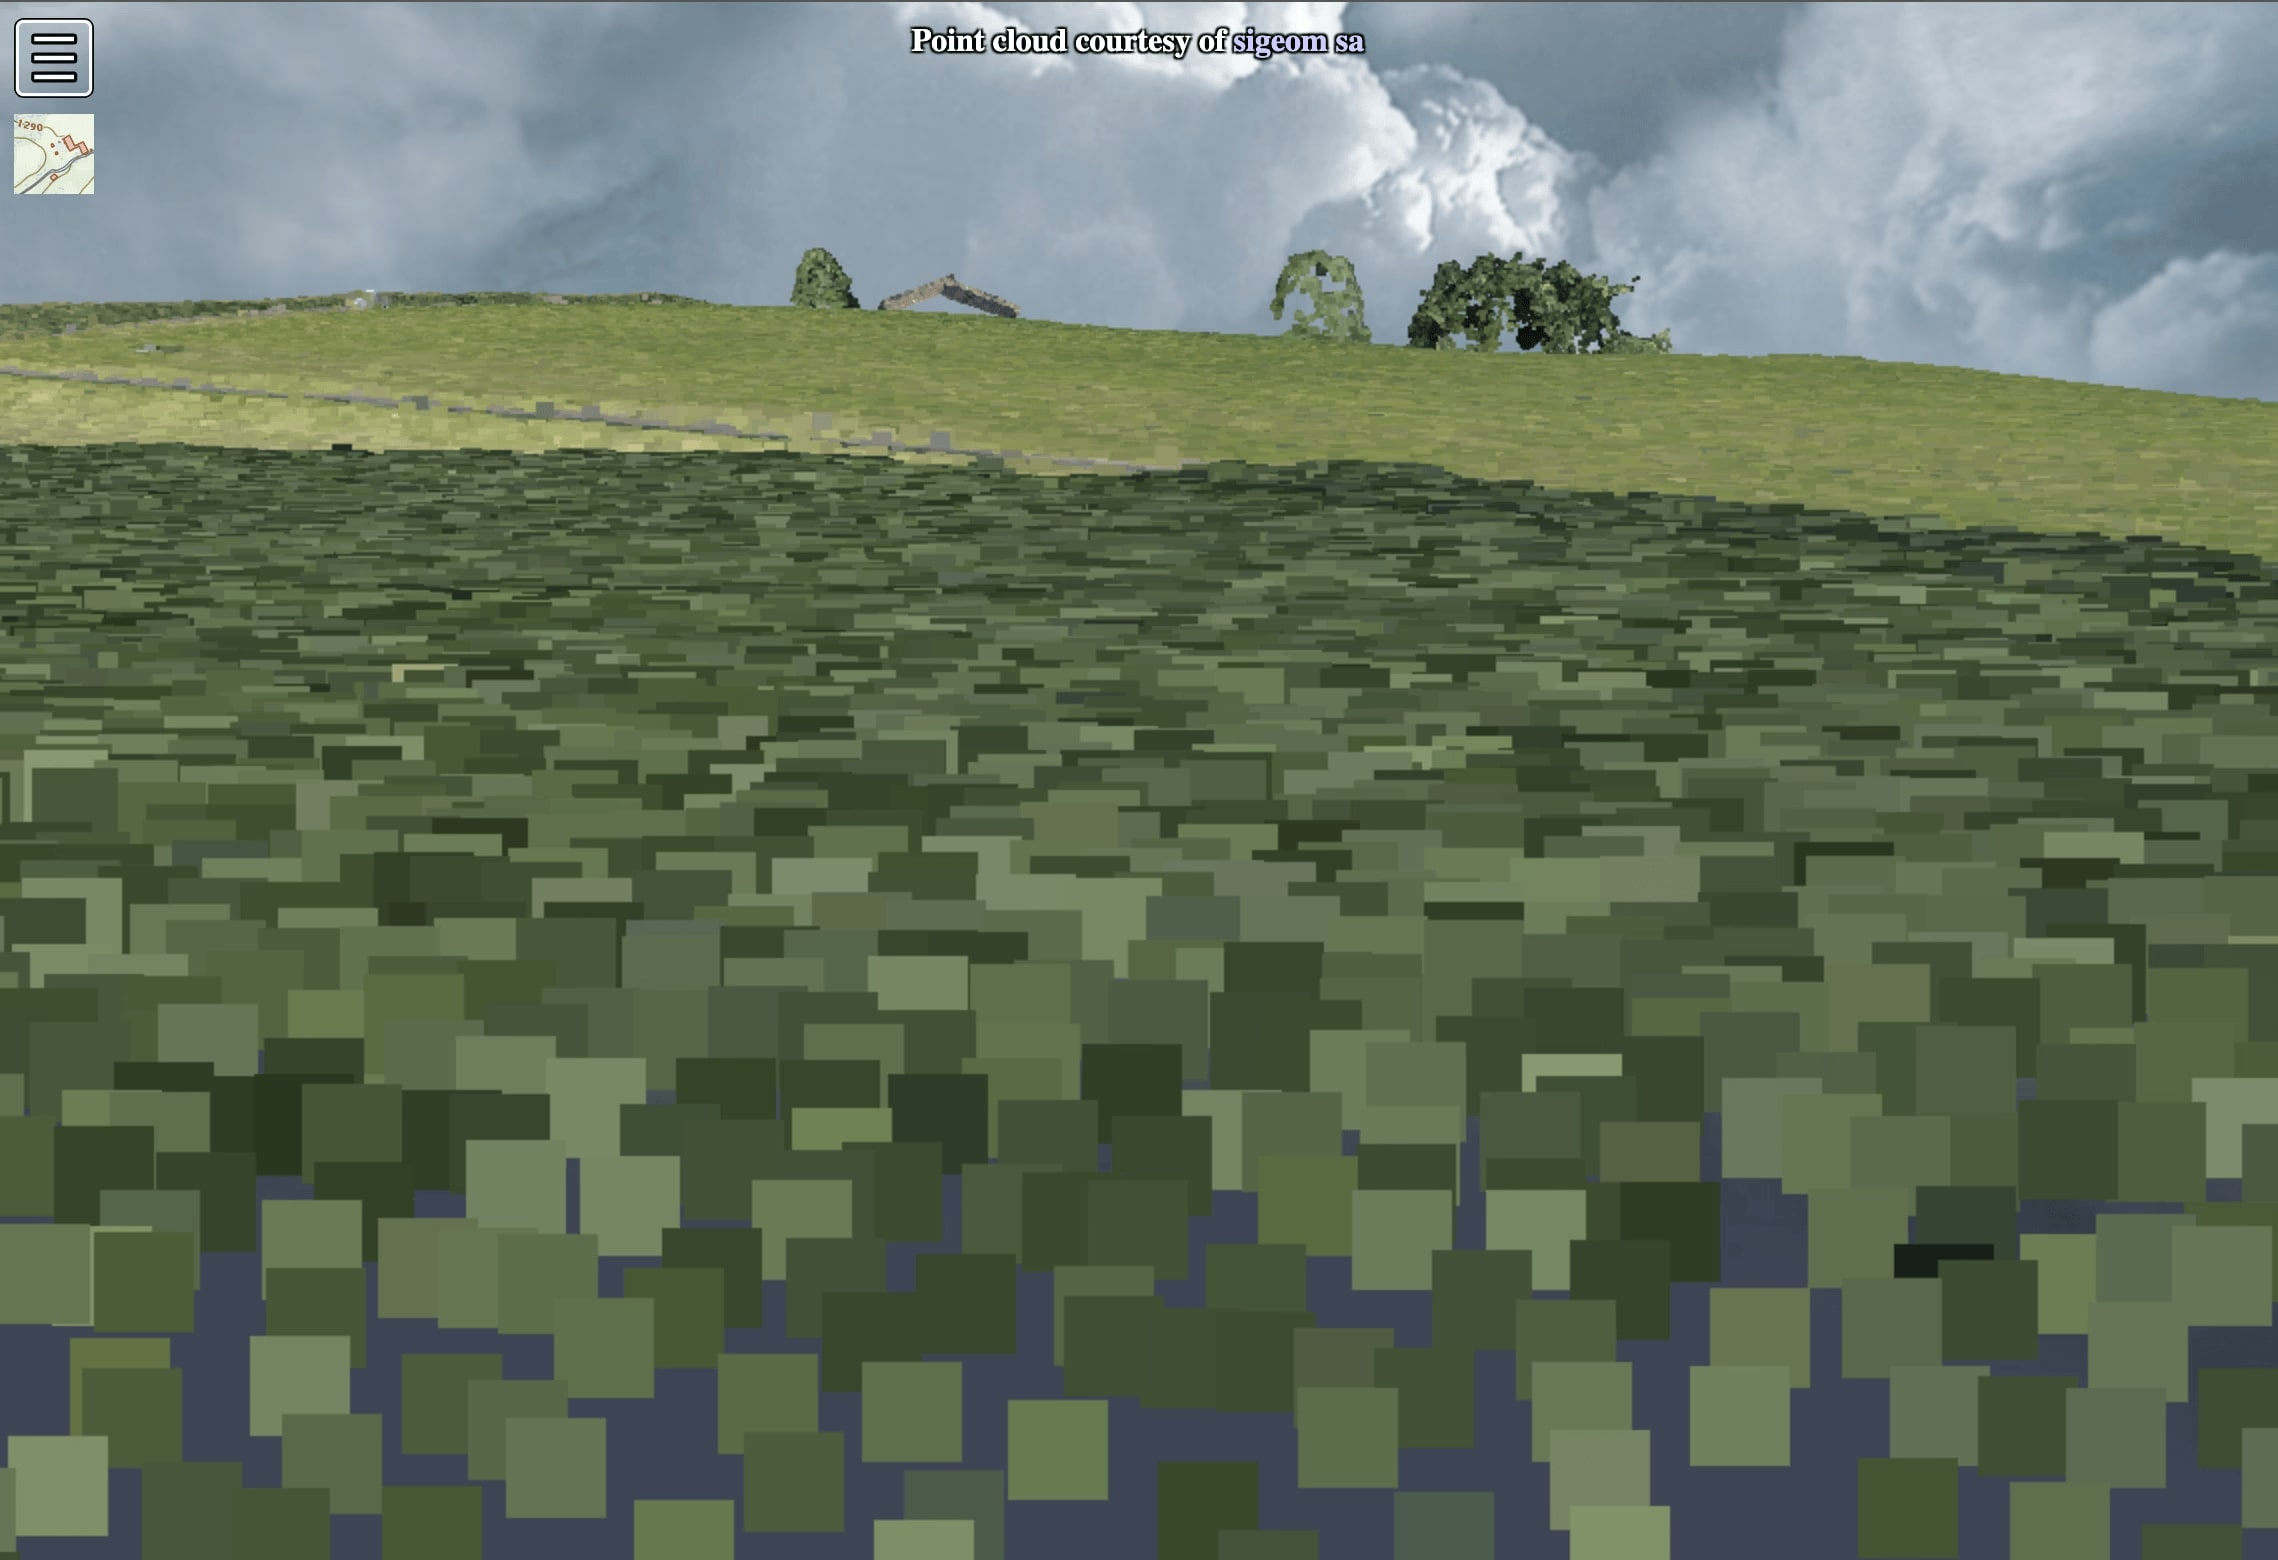
\includegraphics[width=\linewidth,  trim={80 40 80 40}, clip]{images/points.jpg}
		\caption{Point cloud tradizionale} 
		\label{fig:point_cloud_traditional}
	\end{subfigure}
	\hfill
	\begin{subfigure}{0.45\textwidth}
		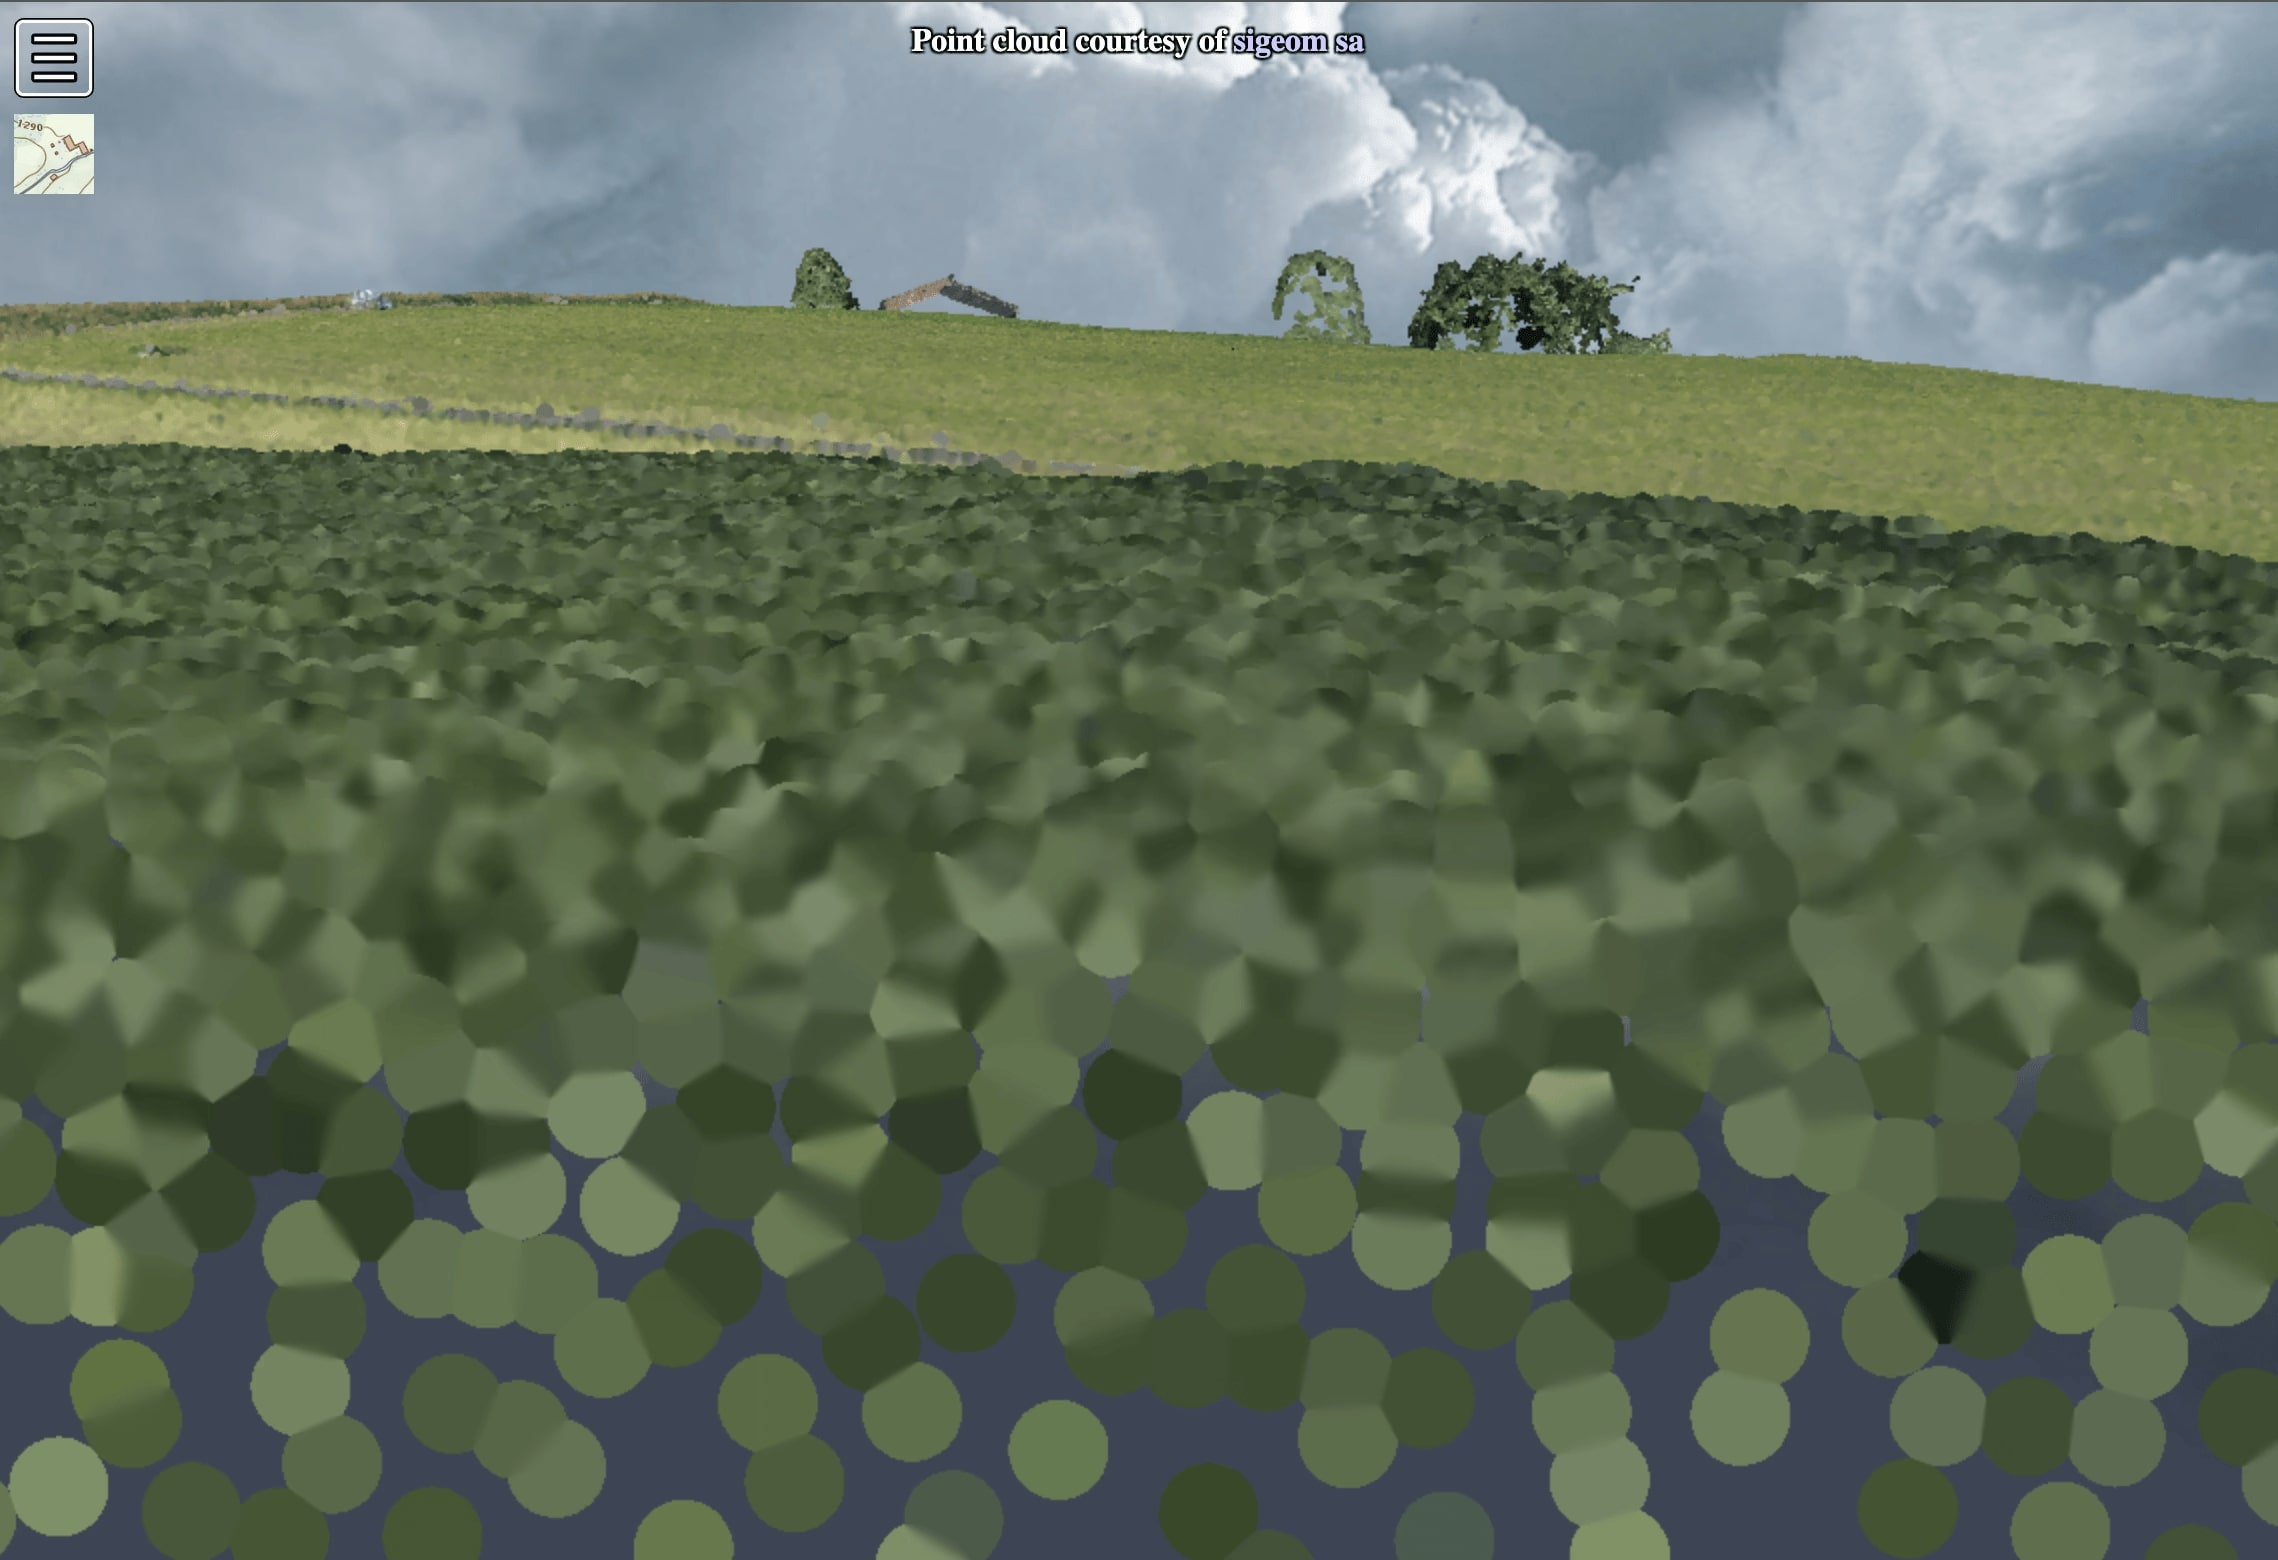
\includegraphics[width=\linewidth, trim={80 40 80 40}, clip]{images/splats.jpg}
		\caption{Point cloud con splatting}  
		\label{fig:point_cloud_with_splatting}
	\end{subfigure}
	\caption{Confronto tra point cloud tradizionale e splatting} \cite{point_cloud_traditional}, \cite{point_cloud_with_splatting}
	\label{fig:comparison_point_clouds}
	,
\end{figure}


\paragraph{Primitive gaussiane come building blocks
}
Una \textbf{gaussiana 3D} può essere concettualizzata come un ellissoide tridimensionale che rappresenta un "pennellata" nello spazio 3D con proprietà variabili. A differenza dei triangoli utilizzati nelle mesh tradizionali o dei punti discreti delle point cloud, le gaussiane offrono una rappresentazione continua e flessibile che può adattarsi a diverse forme geometriche.
\newline
\newline
Ogni gaussiana 3D è definita da un insieme di parametri fondamentali:
\begin{itemize}
\item \textbf{Posizione media $\mu$}: Le coordinate XYZ del centro della gaussiana nello spazio tridimensionale
\item \textbf{Matrice di covarianza $\Sigma$}: Una matrice 3×3 che definisce la forma, le dimensioni e l'orientamento dell'ellissoide gaussiano
\item \textbf{Opacità $\alpha$}: Il grado di trasparenza della primitiva, cruciale per il blending tra gaussiane sovrapposte
\item \textbf{Colore dipendente dalla vista}: Valori RGB che possono essere view-dependent attraverso l'uso di armoniche sferiche
\end{itemize}

\newpage
La funzione gaussiana 3D è espressa come:

\begin{equation}
G(x) = \exp\left(-\frac{1}{2}(x-\mu)^T\Sigma^{-1}(x-\mu)\right)
\end{equation}

\paragraph{Vantaggi della rappresentazione gaussiana}\mbox{}\\
La scelta delle gaussiane come primitive presenta diversi vantaggi significativi:

\begin{itemize}
    \item \textbf{Compattezza rappresentativa}: Scene complesse possono essere rappresentate con 1-5 milioni di gaussiane, mentre point cloud equivalenti potrebbero richiedere decine di milioni o miliardi di punti per la stessa qualità visiva.

    \item \textbf{Fotorealismo}: Le gaussiane permettono di ottenere risultati visivi estremamente realistici, catturando dettagli sottili di illuminazione, ombre e riflessi che spesso mancano in altre rappresentazioni 3D.
    
    \item \textbf{Rappresentazione di geometrie complesse}: A differenza delle mesh che faticano con superfici non-manifold\footnote{Una superficie è \emph{manifold} se l'intorno di ogni punto è topologicamente equivalente a un disco e ogni spigolo è condiviso da esattamente due facce. Esempi di geometrie \emph{non-manifold} includono: spigoli condivisi da tre o più facce, vertici \emph{bow-tie}, giunzioni a T e lamine di spessore nullo.} o topologie complesse, le gaussiane possono rappresentare naturalmente geometrie intricate, dettagli fini e strutture organiche.
    
    \item \textbf{Proprietà anisotrope}: Le gaussiane possono avere valori diversi quando osservate da direzioni diverse. Questa anisotropia, implementata attraverso armoniche sferiche, consente sia di rappresentare strutture geometriche sottili (come fili d'erba o capelli) che di catturare effetti ottici realistici come riflessi che cambiano con il punto di vista.
\end{itemize}
\begin{figure}[htbp]
    \centering
    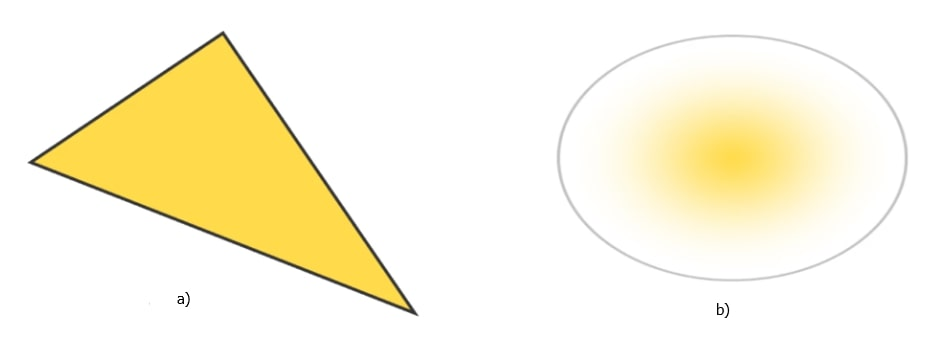
\includegraphics[width=0.9\textwidth]{images/gaussiana_vs_triangle.jpg}
    \caption{Due diverse primitive: a) triangolo b) gaussiana}
    \label{fig:gaussian_and_triangle_mesh}
\end{figure}


\subsection{Pipeline di training}
Il processo di creazione di una rappresentazione Gaussian Splatting segue una pipeline strutturata che trasforma immagini o video di input in un insieme ottimizzato di gaussiane 3D.
La pipeline è così strutturata:
\begin{enumerate}
    \item \textbf{Structure from Motion (SfM)}: Il processo inizia con l'analisi delle immagini di input utilizzando tecniche di Structure from Motion\footnote{La \textit{Structure from Motion} (SfM) è una tecnica di visione artificiale che ricostruisce la geometria tridimensionale di una scena e le traiettorie della camera a partire da immagini bidimensionali multiple, sfruttando la parallasse tra viste. Per un approfondimento si rimanda alla sezione 1.4.}. È necessario che le immagini abbiano sovrapposizione adeguata e coprano la scena da angolazioni diverse. Questa fase genera una point cloud sparsa e stima le pose delle camere, fornendo la struttura geometrica iniziale della scena.

    \item \textbf{Inizializzazione delle gaussiane}: Ogni punto della point cloud sparsa viene successivamente convertito in una gaussiana 3D. Ogni gaussiana viene inizializzata con la posizione del punto corrispondente, il colore derivato dalle osservazioni delle camere, e parametri geometrici di default (covarianza isotropa e opacità iniziale).
    
    \item \textbf{Ottimizzazione differenziabile}: Il cuore del training consiste nell'ottimizzazione dei parametri gaussiani attraverso \textbf{Stochastic Gradient Descent (SGD)}. SGD è un algoritmo di ottimizzazione che trova iterativamente i parametri del modello che minimizzano la differenza tra risultati predetti e target reali.\newline
    A ogni iterazione, il processo seleziona una singola immagine dal dataset di training e confronta l'immagine renderizzata dalla rappresentazione gaussiana corrente con questa immagine target, calcolando una loss function $\mathcal{L}$ che combina:
        \begin{itemize}
            \item \textbf{$\mathcal{L}_1$ (L1 loss)}: misura la differenza assoluta tra pixel corrispondenti delle immagini
            \item \textbf{$\mathcal{L}_{\text{D-SSIM}}$ (Structural Dissimilarity)}: valuta la similarità strutturale e percettiva tra le immagini, catturando differenze che l'occhio umano noterebbe meglio della semplice differenza di colore
        \end{itemize}
        La funzione di loss combinata è definita come:
        \begin{equation}
            \mathcal{L} = (1-\lambda)\mathcal{L}_1 + \lambda \mathcal{L}_{\text{D-SSIM}}
        \end{equation}
        
    dove $\lambda$ è un iperparametro (tipicamente 0.2) che bilancia l'importanza tra accuratezza del colore e similarità strutturale: $\mathcal{L}_1$ garantisce l'accuratezza dei colori di base, che è più critica per la convergenza dell'ottimizzazione rispetto ai dettagli strutturali catturati da D-SSIM.
    L'algoritmo varia i parametri della gaussiane (posizione, colore, forma, dimensione e trasparenza) basandosi su questa funzione di loss.
    
    \item \textbf{Controllo adattivo della densità}: Durante il training, il sistema implementa strategie di densificazione e pruning per ottimizzare il numero e la distribuzione delle gaussiane. Quando una regione è sotto-rappresentata, le gaussiane vengono duplicate (cloning) o suddivise (splitting) per catturare dettagli fini. Di contro, gaussiane con opacità molto bassa vengono rimosse per mantenere efficienza computazionale.
\end{enumerate}

\begin{figure}[htbp]
    \centering
    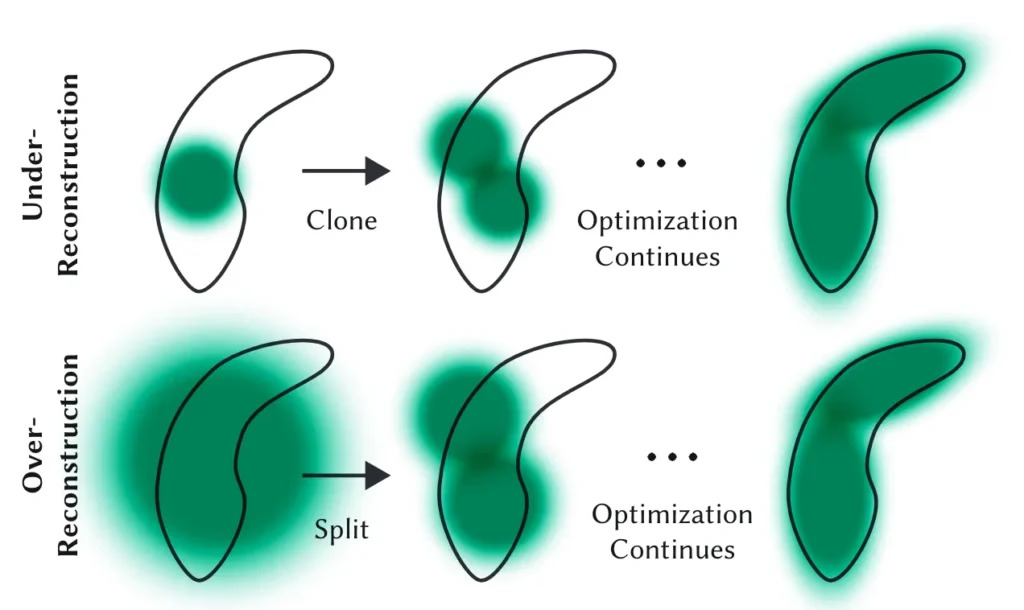
\includegraphics[width=0.9\textwidth]{images/densification.jpg}
    \caption{Densificazione della gaussiane cloning e splitting}
    \label{fig:densification}
\end{figure}

\paragraph{Rasterizzazione differenziabile}
Perché sia possibile l'ottimizzazione descritta sopra, è fondamentale che il processo di rendering sia differenziabile - ovvero che permetta di calcolare come una piccola modifica ai parametri delle gaussiane influenzi il risultato finale dell'immagine renderizzata. Questo collegamento è realizzato attraverso il processo di rasterizzazione differenziabile.
Il rendering delle gaussiane 3D avviene attraverso un processo di rasterizzazione tile-based ottimizzato per hardware GPU, composto dai seguenti passaggi:

\begin{enumerate}
    \item \textbf{Proiezione e ordinamento}: Le gaussiane 3D vengono proiettate sul piano immagine 2D dalla prospettiva della camera. Successivamente, il sistema suddivide lo schermo in tile di 16×16 pixel e raggruppa le gaussiane per tile in base alla loro posizione proiettata.
    \item \textbf{Sorting per depth}: All'interno di ogni tile, le gaussiane vengono ordinate per profondità (distanza dal piano dell'immagine), permettendo un corretto alpha-blending front-to-back durante il rendering.
    \item \textbf{Alpha-blending ottimizzato}: Per ogni pixel, il sistema esegue alpha-blending\footnote{L'\textit{alpha-blending} è una tecnica di compositing che combina più colori in base alla loro opacità (canale alpha), producendo effetti di trasparenza graduata.} delle gaussiane ordinate, combinando i loro contributi di colore e opacità. Questo processo genera gradienti smooth e permette la rappresentazione di superfici continue e effetti di trasparenza complessi.
\end{enumerate}

Il processo di rasterizzazione è completamente differenziabile, permettendo la propagazione dei gradienti attraverso l'intera pipeline di rendering per l'ottimizzazione end-to-end.

\paragraph{View-dependent rendering}
Una caratteristica distintiva del Gaussian Splatting è la capacità di rappresentare effetti ottici che dipendono dalla direzione di osservazione. Questo viene ottenuto attraverso l'uso di \textbf{armoniche sferiche (Spherical Harmonics, SH).}
\newline
\newline
Ogni gaussiana memorizza coefficienti di armoniche sferiche che modulano il colore in base alla direzione di vista. Questa rappresentazione permette di catturare fenomeni come:

\begin{itemize}
    \item Riflessi speculari su superfici lucide
    \item Variazioni di colore dovute a materiali anisotropi
    \item Effetti di illuminazione complessi
    \item Proprietà ottiche direzionali dei materiali
\end{itemize}

\subsection{Strutture dati per gaussiane 3D}

Ogni gaussiana 3D richiede la memorizzazione di diversi parametri:
\begin{itemize}
    \item \textbf{Posizione}: 3 coordinate float (12 bytes)
    \item \textbf{Rotazione}: 4 componenti quaternion (16 bytes)
    \item \textbf{Scala}: 3 valori per gli assi dell'ellissoide (12 bytes)
    \item \textbf{Opacità}: 1 valore alpha (4 bytes)
    \item \textbf{Coefficienti SH}: Variabili in base al grado delle armoniche sferiche (tipicamente 48-192 bytes)
\end{itemize}

Una singola gaussiana richiede quindi circa 92-236 bytes, e con rappresentazioni contenenti 1-5 milioni di gaussiane, i dataset possono facilmente raggiungere centinaia di MB o diversi GB.

\subsubsection{Considerazioni per applicazioni web}

Due fattori critici influenzano l'implementazione web:

\begin{itemize}
\item \textbf{Tempi di caricamento}: La dimensione dei dataset può variare significativamente. Scene semplici possono richiedere 50-100 MB, mentre scene complesse possono superare i 2-6 GB. Per applicazioni web, tempi di download prolungati compromettono l'esperienza utente.

\item \textbf{Performance di rendering}: Le prestazioni sono misurate in FPS (frames per second), con l'obiettivo di mantenere ≥30 FPS per interazioni fluide. La variabilità dell'hardware utente (da dispositivi mobili economici a workstation grafiche) richiede strategie di ottimizzazione adattive.
\end{itemize}
\subsubsection{Formati e ottimizzazioni}
La rappresentazione GSplat, essendo concettualmente simile alle point cloud,
utilizza formati di file che riflettono questa affinità. Il formato più comune-
mente adottato è il PLY (.ply), un formato standard ampiamente utilizzato
per la memorizzazione di dati geometrici 3D. Questo formato si adatta natu-
ralmente alla struttura dei dati gaussiani, permettendo di memorizzare tutti
i parametri essenziali di ogni gaussiana: posizione, matrice di covarianza,
opacità e coefficienti delle armoniche sferiche per il colore view-dependent.
Parallelamente allo sviluppo della tecnologia GSplat, la comunità open sour-
ce sta creando formati specializzati come .splat e .ksplat (versione compressa), ottimizzati specificamente per le caratteristiche uniche delle gaussiane 3D. Questo è un campo in rapida evoluzione, con nuovi formati che
emergono continuamente per rispondere alle esigenze specifiche di diverse
applicazioni.
Tuttavia, per applicazioni web potrebbero essere necessarie una o più delle seguenti ottimizzazioni:

\begin{itemize}
    \item \textbf{Compressione}: Tecniche di quantizzazione per ridurre la precisione floating-point mantenendo qualità visiva
    \item \textbf{Streaming progressivo}: Caricamento incrementale per visualizzazione immediata con raffinamento graduale
    \item \textbf{Level-of-Detail (LOD)}: Rappresentazioni multiple a diverse risoluzioni per adattarsi alle capacità hardware
    \item \textbf{Culling spaziale}: Eliminazione di gaussiane non visibili per ridurre il carico computazionale
\end{itemize}

Queste considerazioni sono fondamentali per lo sviluppo di piattaforme accessibili che rendano il 3D Gaussian Splatting fruibile su una vasta gamma di dispositivi e connessioni di rete.
\subsection{Posizionamento nel panorama delle tecniche attuali}
Il 3D Gaussian Splatting si posiziona come soluzione ibrida che combina vantaggi di diverse famiglie di tecniche di rappresentazione 3D.
\newline
\newline
\textbf{Rispetto alle mesh tradizionali}: Mentre le mesh eccellono nella rappresentazione di superfici ben definite e sono ottimizzate per pipeline di rendering consolidate, il Gaussian Splatting offre maggiore flessibilità per fenomeni volumetrici e materiali trasparenti, pur mantenendo efficienza di rendering comparabile.
\newline
\newline
\textbf{Rispetto ai Neural Radiance Fields}: NeRF utilizza reti neurali per rappresentare implicitamente radiance field volumetrici, ottenendo alta qualità visiva ma richiedendo tempi di rendering significativamente più lunghi (secondi per frame). Il Gaussian Splatting raggiunge qualità visiva comparabile con velocità di rendering real-time ($\geq$ 30 FPS), eliminando la necessità di query neurali durante il rendering.
\newline
\newline
\textbf{Rispetto alle point cloud}: Condividendo la natura di dati non strutturati, il Gaussian Splatting supera le limitazioni delle point cloud tradizionali attraverso primitive più espressive (ellissoidi vs punti) e capacità di rappresentare continuità spaziale e effetti ottici complessi.

\paragraph{Innovazioni architetturali}
Il successo del Gaussian Splatting deriva da diverse innovazioni tecniche chiave:
\begin{itemize}
    \item \textbf{Rasterizzazione tile-based}: L'approccio di suddivisione in tile riduce significativamente la complessità computazionale del sorting e dell'alpha-blending, rendendo possibile il rendering real-time di milioni di gaussiane.
    \item \textbf{Differenziabilità end-to-end}: L'intera pipeline, dalla rappresentazione 3D al rendering 2D, è completamente differenziabile, permettendo ottimizzazione diretta tramite gradient descent senza approssimazioni.
    \item \textbf{Controllo adattivo automatico}: Il sistema di densificazione e pruning automatico permette di bilanciare dinamicamente qualità visiva e efficienza computazionale durante il training.
\end{itemize}
Queste caratteristiche posizionano il 3D Gaussian Splatting come tecnica particolarmente adatta per applicazioni che richiedono il bilanciamento di alta qualità visiva, efficienza computazionale e tempi di training ragionevoli, rendendolo ideale per lo sviluppo di piattaforme accessibili come quella proposta in questo lavoro.

\section{Structure from Motion e COLMAP: prerequisiti per 3D Gaussian Splatting}

Prima di fornire una panoramica sugli algoritmi coinvolti nella realizzazione di questo specifico progetto, è fondamentale comprendere il processo di preprocessing che rende possibile l'applicazione di queste tecniche. Tutti gli algoritmi di 3DGS, indipendentemente dalle loro specifiche implementazioni, condividono un requisito comune: la necessità di una nuvola di punti 3D iniziale e delle pose precise delle camere per ogni immagine di input. Questi dati vengono tipicamente generati attraverso tecniche di Structure from Motion (SfM), con COLMAP che rappresenta lo standard de facto per questa fase di preprocessing.

\subsection{Structure from Motion: ricostruzione 3D da immagini}

Structure from Motion (SfM) è una famiglia di algoritmi di computer vision che permette di ricostruire la struttura tridimensionale di una scena e le posizioni delle camere a partire da una collezione di immagini bidimensionali non ordinate. Il principio fondamentale si basa sulla geometria epipolare: quando lo stesso punto fisico viene osservato da due o più posizioni differenti, è possibile triangolare la sua posizione nello spazio 3D utilizzando i principi della geometria proiettiva.

Il processo SfM può essere sintetizzato in tre fasi principali. Inizialmente, vengono estratti punti caratteristici (feature) da ogni immagine utilizzando algoritmi come SIFT, SURF o ORB. Successivamente, questi punti vengono messi in corrispondenza tra immagini diverse per identificare lo stesso punto fisico osservato da angolazioni multiple. Infine, utilizzando queste corrispondenze, viene ricostruita simultaneamente la struttura 3D della scena e le pose delle camere attraverso tecniche di ottimizzazione non lineare.

\noindent L'output di un algoritmo SfM consiste tipicamente in una nuvola di punti 3D sparsa che rappresenta i punti caratteristici della scena, le pose delle camere (posizione e orientamento) per ogni immagine, e i parametri intrinseci delle camere (lunghezza focale, centro ottico, distorsioni). Questa rappresentazione sparsa, pur non catturando completamente la geometria della scena, fornisce una base solida per tecniche di ricostruzione più dense come il 3D Gaussian Splatting.

\begin{figure}[htbp]
    \centering
    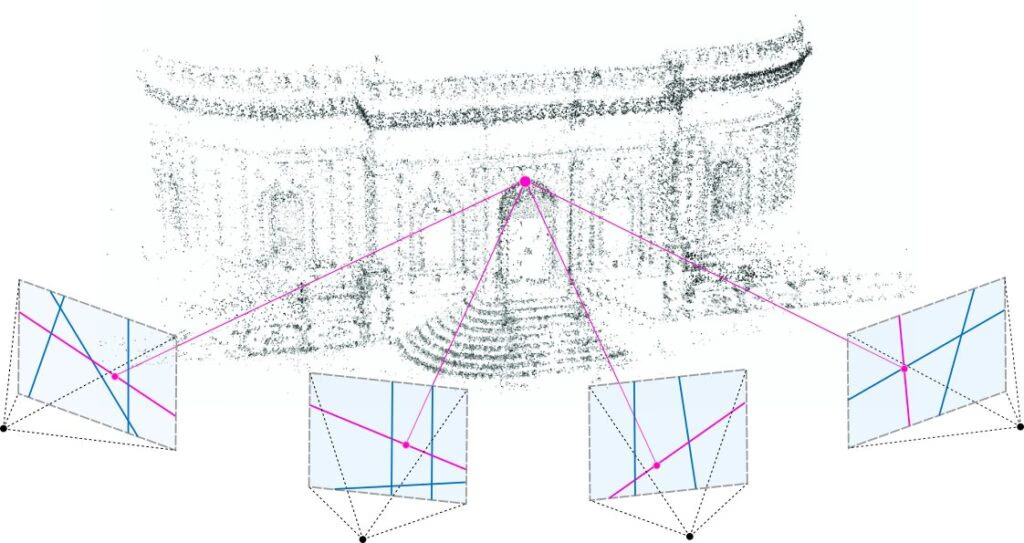
\includegraphics[width=0.9\textwidth]{images/sfm.jpg}
    \caption{Rappresentazione del concetto di Structure From Motion}
    \label{fig:sfm}
    Fonte: \cite{sfm}
\end{figure}
\subsection{COLMAP: implementazione di riferimento per SfM}

COLMAP (COLlaborative Large-scale universal MApping and Positioning) è un framework open-source per Structure from Motion e Multi-View Stereo sviluppato presso l'ETH Zurich. Rappresenta una delle implementazioni più robuste e complete di algoritmi SfM, combinando efficienza computazionale con accuratezza geometrica. COLMAP è diventato lo standard de facto nella comunità di computer vision per la ricostruzione 3D da immagini, supportando una vasta gamma di scenari applicativi.

La pipeline COLMAP implementa un approccio incrementale alla ricostruzione, iniziando con una coppia di immagini ben condizionata e aggiungendo progressivamente nuove viste. Questo metodo garantisce robustezza anche in presenza di scene complesse o dati di input rumorosi. Il sistema integra automaticamente tecniche di bundle adjustment\footnote{Il \emph{bundle adjustment} è una tecnica di ottimizzazione non lineare che raffina simultaneamente tutti i parametri della ricostruzione 3D (posizioni dei punti, pose delle camere e parametri intrinseci) minimizzando l'errore di riproiezione tra i punti ricostruiti e le loro osservazioni nelle immagini.} per l'ottimizzazione simultanea di tutti i parametri, gestione intelligente degli outlier\footnote{Gli \emph{outlier} sono dati errati o rumorosi che non seguono il modello geometrico della scena, come corrispondenze sbagliate tra feature o punti 3D mal triangolati, che devono essere identificati e rimossi per garantire l'accuratezza della ricostruzione.}, e supporto per diversi modelli di camera e condizioni di acquisizione.

Una caratteristica distintiva di COLMAP è la sua capacità di gestire automaticamente molte delle complessità tipiche della ricostruzione SfM, come la selezione delle immagini di inizializzazione, la gestione di scene con componenti disconnesse, e l'identificazione di loop closure\footnote{La \emph{loop closure} è il riconoscimento che la camera è tornata in una posizione già visitata, fondamentale per correggere la deriva accumulata durante la ricostruzione incrementale e migliorare la coerenza globale della scena ricostruita.} in sequenze di immagini. Queste funzionalità rendono COLMAP particolarmente adatto come preprocessing per applicazioni downstream come il 3D Gaussian Splatting.

\subsection{Integrazione COLMAP-3DGS: dal preprocessing al rendering}

La connessione tra COLMAP e 3D Gaussian Splatting è fondamentale e bidirezionale. COLMAP fornisce i dati di input essenziali per tutti gli algoritmi 3DGS, mentre la qualità della ricostruzione COLMAP determina direttamente le prestazioni achievable dai metodi di Gaussian Splatting.

L'output principale di COLMAP utilizzato da 3DGS è la nuvola di punti 3D sparsa, dove ogni punto viene utilizzato per inizializzare una gaussiana 3D. Le coordinate del punto diventano la posizione media della gaussiana, mentre parametri come scala, rotazione e opacità vengono inizializzati utilizzando euristiche. Inoltre, COLMAP fornisce le pose precise delle camere, indispensabili per il processo di rendering differenziabile che costituisce il cuore dell'ottimizzazione 3DGS.

La qualità della ricostruzione COLMAP influenza profondamente le prestazioni finali del sistema 3DGS. Una nuvola di punti densa e accurata fornisce una migliore inizializzazione, riducendo il tempo di convergenza e migliorando la qualità finale. Di contro, errori nella stima delle pose delle camere o nella triangolazione dei punti 3D si propagano attraverso l'intero processo di training, limitando la fedeltà del rendering finale.

È importante notare che COLMAP ricostruisce tipicamente solo i punti più caratteristici e facilmente triangolabili della scena, risultando in una rappresentazione sparsa. Aree uniformi, superfici riflettenti, o regioni con texture insufficiente potrebbero non essere rappresentate nella nuvola di punti iniziale. Questa limitazione è uno dei motivi per cui gli algoritmi 3DGS includono meccanismi di densificazione adattiva durante il training, per colmare le lacune nella rappresentazione iniziale.

\subsection{Requisiti e limitazioni}

Per ottenere risultati di qualità con la pipeline COLMAP-3DGS, è necessario rispettare alcuni requisiti fondamentali nella fase di acquisizione dati. Le immagini devono presentare un overlap sufficiente (tipicamente 60-80\% tra immagini adiacenti) per garantire corrispondenze robuste. La scena deve contenere texture sufficienti per la feature detection, ed è preferibile mantenere condizioni di illuminazione consistenti durante l'acquisizione.

Le limitazioni principali riguardano scene con caratteristiche problematiche per gli algoritmi SfM: superfici uniformi o riflettenti che non generano feature distintive, pattern ripetitivi che possono causare corrispondenze errate, e variazioni di illuminazione drastiche che influenzano la consistenza delle feature. Inoltre, COLMAP, come tutti gli algoritmi SfM, richiede che la scena sia statica durante l'acquisizione.

Nonostante queste limitazioni, la combinazione COLMAP-3DGS rappresenta attualmente la soluzione più matura e affidabile per la generazione di radiance field di alta qualità a partire da immagini multi-vista. La robustezza di COLMAP nella fase di preprocessing, combinata con la capacità dei metodi 3DGS di densificare e raffinare la rappresentazione durante il training, permette di ottenere risultati di qualità eccellente su una vasta gamma di scene reali.

La comprensione di questa pipeline integrata è essenziale per l'utilizzo efficace delle tecniche di 3D Gaussian Splatting, poiché la qualità del preprocessing COLMAP costituisce spesso il fattore limitante per le prestazioni complessive del sistema.

\section{Algoritmi di training utilizzati}

\subsection{Approccio standard (3DGS baseline)}

L'implementazione originale di Kerbl et al. si basa su un approccio di ottimizzazione diretta mediante gradient descent, dove ogni gaussiana 3D viene parametrizzata attraverso posizione, covarianza (scala e rotazione), opacità e coefficienti delle armoniche sferiche per il colore. Il processo di training alterna fasi di ottimizzazione dei parametri gaussiani con operazioni di controllo della densità (densificazione e pruning) per adattare dinamicamente la rappresentazione alla complessità della scena. Questo approccio rappresenta il metodo standard e più consolidato, caratterizzato da semplicità implementativa e robustezza.

\paragraph{Vantaggi chiave}
\begin{itemize}
	\item Risultati stabili e riproducibili
	\item Requisiti hardware accessibili
	\item Buon bilanciamento qualità/prestazioni per scene standard
\end{itemize}

\paragraph{Svantaggi}
\begin{itemize}
	\item Tendenza a generare artefatti "needle-like" in alcune configurazioni
	\item Gestione non ottimale nella distribuzione delle Gaussiane
	\item Difficoltà in scene molto complesse o dense
	\item Controllo limitato sull'allocazione automatica delle risorse
	\item Tendenza a stabilizzarsi in configurazioni subottimali della scena, tipico dei metodi ottimizzati per gradient descent locale
\end{itemize}

\subsection{Monte Carlo Markov Chain: miglioramento qualità tramite campionamento probabilistico}

Il metodo MCMC (Monte Carlo Markov Chain), applicato al training delle Gaussiane 3D, rappresenta un'estensione del metodo originale proposto nel paper fondamentale di 3D Gaussian Splatting. Questo approccio avanzato utilizza una variante chiamata \textbf{Stochastic Gradient Langevin Dynamics (SGLD)} per campionare le configurazioni delle primitive da una distribuzione target, introducendo un rumore stocastico controllato che permette una migliore esplorazione dello spazio delle soluzioni e previene il collasso in minimi locali. Il framework MCMC eredita tutti i parametri in input già elencati in precedenza e ne introduce di aggiuntivi in modo da sfruttare strategie di ottimizzazione più sofisticate.

Inoltre, il metodo include un meccanismo di regolazione della complessità del modello, che consente di controllare dinamicamente il numero di Gaussiane attive durante il training, con l'obiettivo di bilanciare efficacia della rappresentazione e uso efficiente delle risorse computazionali. Questa estensione affronta specificamente alcune limitazioni del metodo originale, come la distribuzione spaziale non ottimale delle Gaussiane e la presenza di Gaussiane "morte" (cioè primitive che cessano di contribuire attivamente al rendering durante il processo di training).

\paragraph{Vantaggi chiave}
\begin{itemize}
	\item Relocazione automatica ed efficace delle Gaussiane non attive
	\item Prevenzione della stagnazione in minimi locali subottimali
	\item Riduzione degli artefatti visivi (needle-like)
	\item Distribuzione spaziale più regolare e adattiva
	\item Migliore esplorazione dello spazio delle soluzioni tramite rumore controllato
\end{itemize}

\paragraph{Svantaggi}
\begin{itemize}
	\item Aumento della complessità implementativa e concettuale
	\item Parametri aggiuntivi da ottimizzare con attenzione
	\item Overhead computazionale dovuto al sampling stocastico
	\item Possibile rallentamento della convergenza se \texttt{noise\_lr} è mal bilanciato
	\item Risultati leggermente meno deterministici a causa dell'introduzione del rumore
\end{itemize}

\subsection{Taming 3DGS: ottimizzazione per risorse computazionali limitate}

Il metodo Taming 3DGS nasce come risposta alle limitazioni computazionali tipiche del Gaussian Splatting su dispositivi non high-end. Il suo contributo principale è l'introduzione di un sistema incrementale e score-guided per la densificazione, in cui ogni nuova Gaussiana viene inserita solo se il suo apporto qualitativo alla scena giustifica il costo computazionale. L'intero processo è regolato da un sistema di punteggio che tiene conto della visibilità, dell'influenza sul gradiente della loss e del contributo alla qualità visiva.

Anche in questo caso, è previsto un sistema di controllo della complessità del modello, che consente di limitare o guidare la crescita del numero di Gaussiane in base a parametri specifici. Questo approccio si traduce in un controllo preciso e prevedibile delle risorse, con implicazioni dirette su tempo, memoria e qualità. L'architettura del metodo evita picchi di memoria durante il training, permettendo la generazione di scene complesse anche su hardware con risorse limitate. Grazie a parametri mirati, è possibile adattare dinamicamente la crescita del modello in funzione della scena e dei vincoli imposti (es. massimo numero di Gaussiane o soglie qualitative minime).
\mbox{}\\
\begin{itemize}
	\item Controllo preciso delle risorse computazionali
	\item Scalabilità su hardware limitato
	\item Processo costruttivo senza picchi di memoria
	\item Densificazione intelligente basata su score
	\item Adattabilità automatica alla complessità della scena
\end{itemize}

\paragraph{Svantaggi}
\begin{itemize}
	\item Possibile perdita di dettagli fini con budget limitati
	\item Complessità aggiuntiva nella configurazione dei parametri
	\item Overhead computazionale per il calcolo degli score
	\item Dipendenza dalla stima accurata dello score di importanza delle gaussiane
	\item Potenziale sottoottimizzazione per rispettare i vincoli di budget
\end{itemize}

\subsection{Parametri di configurazione del training}
I parametri di configurazione permettono di controllare tutti gli aspetti del training nei tre metodi presentati: durata dell'ottimizzazione, gestione delle risorse computazionali e qualità finale del modello. Ogni metodo estende il set di parametri base con opzioni specifiche per le proprie caratteristiche innovative.

I parametri base del 3D Gaussian Splatting (Tabella \ref{tab:3dgs_params}) controllano aspetti fondamentali come numero di iterazioni, risoluzione e densificazione. Il metodo MCMC aggiunge parametri di regolarizzazione (Tabella \ref{tab:mcmc_params}), mentre Taming 3DGS introduce controlli specifici per la gestione delle risorse (Tabella \ref{tab:taming_params}). Le tabelle complete con tutti i parametri e i loro effetti sono riportate nell'Appendice \ref{app:parametri}.


\subsection{Confronto degli approcci}

\begin{table}[h]
	\centering
	\small
	\begin{tabular}{|l|c|c|c|}
		\hline
		\textbf{Criterio} & \textbf{3DGS} & \textbf{MCMC} & \textbf{Taming} \\
		\hline
		Qualità risultato & Buona & Superiore & Adattabile al budget \\
		\hline
		Velocità training & Veloce & Moderata (overhead) & Veloce \\
		\hline
		Uso memoria & Variabile & Controllato & Predicibile \\
		\hline
		Complessità impl. & Bassa & Alta (catena MCMC) & Moderata \\
		\hline
		Requisiti HW & Moderati & Moderati–Alti & Flessibili \\
		\hline
		Stabilità risultati & Alta & Moderata & Alta \\
		\hline
		Controllo risorse & Limitato & Moderato & Eccellente \\
		\hline
	\end{tabular}
	\caption{Confronto tra metodi}
\end{table}

\paragraph{Raccomandazioni d'uso}
\begin{itemize}
	\item \textbf{3DGS Standard}: ideale per applicazioni standard, prototipazione rapida e quando la semplicità implementativa è prioritaria
	\item \textbf{3DGS MCMC}: consigliato per scene complesse dove la qualità è critica e si dispone di risorse computazionali adeguate
	\item \textbf{Taming 3DGS}: ottimale per deployment su hardware limitato, applicazioni real-time e quando il controllo delle risorse è fondamentale
\end{itemize}

\newpage

\section{Metriche di Valutazione}
La valutazione quantitativa della qualità dei modelli 3D generati tramite tecniche di rendering neurale rappresenta una sfida fondamentale nel campo della computer vision. A differenza delle tecniche tradizionali di modellazione 3D, dove la valutazione può concentrarsi su aspetti puramente geometrici, i metodi basati su Gaussian Splatting richiedono metriche che catturino sia la fedeltà visiva che la percezione umana del realismo.

\subsection{Peak Signal-to-Noise Ratio (PSNR)}
Il PSNR rappresenta la metrica più diffusa per la valutazione pixel-wise della qualità di immagini ricostruite. Definito come il rapporto logaritmico tra il valore massimo possibile del segnale e la potenza del rumore di distorsione, il PSNR fornisce una misura oggettiva della fedeltà della ricostruzione:

\begin{equation}
	\text{PSNR} = 10 \cdot \log_{10}\left(\frac{\text{MAX}^2}{\text{MSE}}\right)
\end{equation}

dove MAX rappresenta il valore massimo possibile dei pixel (tipicamente 255 per immagini a 8 bit) e MSE è l'errore quadratico medio tra l'immagine di riferimento e quella ricostruita.

Nel contesto del Gaussian Splatting, il PSNR viene calcolato confrontando le immagini renderizzate dal modello 3D con le immagini ground truth\footnote{Il termine \emph{ground truth} indica i dati di riferimento considerati corretti e accurati, utilizzati come standard per valutare le prestazioni di un algoritmo o modello. Nel contesto del Gaussian Splatting, si riferisce alle immagini originali del dataset di acquisizione.} del dataset di test. Valori più elevati di PSNR indicano una maggiore fedeltà della ricostruzione, con soglie tipiche che considerano acceptable ricostruzioni con PSNR superiore a 20-25 dB per scene complesse.\newline
Nonostante la sua diffusione, il PSNR presenta limitazioni significative nella valutazione della qualità percettiva. La metrica non tiene conto della struttura locale delle immagini né delle caratteristiche del sistema visivo umano, risultando spesso inadeguata per catturare aspetti qualitativi importanti come la nitidezza dei dettagli o la coerenza delle texture.

\subsection{Structural Similarity Index Measure (SSIM)}

Lo SSIM, introdotto da Wang et al., rappresenta un approccio più sofisticato alla valutazione della qualità delle immagini, progettato per correlare meglio con la percezione visiva umana. La metrica opera attraverso la valutazione separata di tre componenti fondamentali del sistema visivo umano, che vengono successivamente combinate in un singolo indice di qualità:

\begin{equation}
	\text{SSIM}(x,y) = [l(x,y)]^{\alpha} \times [c(x,y)]^{\beta} \times [s(x,y)]^{\gamma}
\end{equation}

dove $l(x,y)$, $c(x,y)$ e $s(x,y)$ rappresentano rispettivamente la componente di luminanza, contrasto e struttura, con esponenti $\alpha$, $\beta$, $\gamma$ per controllare l'importanza relativa di ciascuna componente.

I tre componenti sono definiti come:\newline

\textbf{Luminanza}:
\begin{equation}
	l(x,y) = \frac{2\mu_x\mu_y + c_1}{\mu_x^2 + \mu_y^2 + c_1}
\end{equation}

\textbf{Contrasto}:
\begin{equation}
	c(x,y) = \frac{2\sigma_x\sigma_y + c_2}{\sigma_x^2 + \sigma_y^2 + c_2}
\end{equation}

\textbf{Struttura}:
\begin{equation}
	s(x,y) = \frac{\sigma_{xy} + c_3}{\sigma_x\sigma_y + c_3}
\end{equation}

dove $\mu$ rappresenta la media locale, $\sigma$ la deviazione standard locale, $\sigma_{xy}$ la covarianza locale, e $c_1$, $c_2$, $c_3$ sono costanti di stabilizzazione.\newline
Nella pratica, si utilizza comunemente la versione con $\alpha = \beta = \gamma = 1$ e $c_3 = c_2/2$, che produce la formula compatta:

\begin{equation}
	\text{SSIM}(x,y) = \frac{(2\mu_x\mu_y + c_1)(2\sigma_{xy} + c_2)}{(\mu_x^2 + \mu_y^2 + c_1)(\sigma_x^2 + \sigma_y^2 + c_2)}
\end{equation}

I tre componenti valutano aspetti complementari:
\begin{itemize}
	\item \textbf{Luminanza}: Confronto delle intensità medie locali - misura quanto le due immagini sono simili in termini di brillantezza complessiva
	\item \textbf{Contrasto}: Confronto della varianza delle intensità - valuta se le due immagini hanno simili livelli di dettaglio e texture
	\item \textbf{Struttura}: Confronto dei pattern di correlazione spaziale - cattura la similarità nei pattern geometrici e nelle relazioni spaziali tra pixel
\end{itemize}

Lo SSIM produce valori compresi tra -1 e 1, dove 1 indica identità perfetta. Nel rendering neurale, valori SSIM superiori a 0.8-0.9 sono generalmente considerati indicativi di alta qualità visiva.\newline
La separazione in tre componenti consente di diagnosticare specifici aspetti della qualità dell'immagine. Una ricostruzione può avere buona luminanza e contrasto ma struttura degradata, indicando problemi nella preservazione dei dettagli geometrici tipici nelle scene renderizzate con Gaussian Splatting.

\subsection{Learned Perceptual Image Patch Similarity (LPIPS)}

La metrica LPIPS, sviluppata da Zhang et al., rappresenta l'evoluzione più recente nella valutazione percettiva delle immagini, utilizzando reti neurali pre-addestrate per catturare similarità percettive complesse. A differenza delle metriche tradizionali basate su operazioni matematiche dirette sui pixel, LPIPS sfrutta le rappresentazioni apprese da deep network addestrate su task di computer vision.

La metrica opera estraendo feature da diversi layer di reti convoluzionali (tipicamente VGG, AlexNet, o SqueezeNet) e calcolando la distanza pesata tra le rappresentazioni delle immagini da confrontare:

\begin{equation}
	\text{LPIPS} = \sum_l \frac{1}{H_l W_l} \sum_{h,w} ||\mathbf{w}_l \odot (\mathbf{y}^l_{hw} - \mathbf{y}^{l*}_{hw})||_2^2
\end{equation}

dove $l$ indica i layer della rete, $\mathbf{w}_l$ sono pesi appresi, e $\mathbf{y}^l$ rappresenta le feature normalizzate.

\paragraph{Caratteristiche distintive di LPIPS}
\begin{itemize}
	\item \textbf{Sensibilità percettiva}: Cattura distorsioni rilevanti per la percezione umana che sfuggono a metriche tradizionali
	\item \textbf{Robustezza alle trasformazioni}: Meno sensibile a spostamenti pixel-wise che non alterano la percezione
	\item \textbf{Correlazione con giudizi umani}: Elevata correlazione con valutazioni soggettive di qualità
\end{itemize}

Nel contesto del Gaussian Splatting, LPIPS si rivela particolarmente efficace nel distinguere tra ricostruzioni che, pur avendo PSNR/SSIM simili, presentano differenze qualitative significative in termini di realismo e fedeltà percettiva.

\subsection{Applicazione nel Gaussian Splatting}

\subsubsection{Complementarità delle metriche}

L'utilizzo combinato di PSNR, SSIM e LPIPS fornisce una valutazione multi-dimensionale della qualità dei modelli generati:

\begin{itemize}
	\item \textbf{PSNR}: Valutazione della fedeltà pixel-wise e del rumore complessivo
	\item \textbf{SSIM}: Analisi della preservazione delle strutture locali e della coerenza spaziale  
	\item \textbf{LPIPS}: Valutazione della qualità percettiva e del realismo visivo
\end{itemize}

\subsubsection{Sfide specifiche}

La valutazione dei modelli Gaussian Splatting presenta sfide peculiari, ovvero:

\begin{itemize}
	\item \textbf{View-dependence}: A differenza delle immagini statiche, i modelli 3D devono essere valutati da multiple viewpoint, richiedendo l'aggregazione di metriche su diversi punti di vista.
	\item \textbf{Temporal consistency}: Per sequenze video, è necessario valutare anche la coerenza temporale tra frame consecutivi.
	\item \textbf{Scene complexity}: Scene con elementi trasparenti, riflessi o illuminazione complessa possono presentare trade-off diversi tra le metriche.
\end{itemize}

\subsubsection{Benchmark e soglie di Riferimento}

Nel contesto dei dataset standard per la valutazione del Gaussian Splatting (NeRF Synthetic, Mip-NeRF 360, Tanks and Temples), sono emersi range tipici di valori considerati rappresentativi di alta qualità:

\begin{itemize}
	\item \textbf{PSNR}: 25-35 dB per scene indoor, 20-30 dB per scene outdoor
	\item \textbf{SSIM}: 0.85-0.95 per ricostruzioni di alta qualità
	\item \textbf{LPIPS}: 0.05-0.15 (valori più bassi indicano maggiore similarità percettiva)
\end{itemize}

Questi benchmark forniscono riferimenti fondamentali per valutare l'efficacia di nuove varianti algoritmiche e ottimizzazioni implementative nel campo del Gaussian Splatting.

\section{Applicazioni e limitazioni attuali} 
\subsection{Campi di applicazione nella computer vision}
Il 3D Gaussian Splatting trova applicazione in diversi domini:
\begin{itemize}
	\item \textbf{Novel View Synthesis}: è una tecnica che ha l'obiettivo di generare nuove immagini di una scena da punti di vista non osservati direttamente, a partire da un insieme limitato di viste iniziali, sfruttando informazioni spaziali e fotometriche per garantire realismo e coerenza.
	\item \textbf{Digital Content Creation}: Creazione di asset 3D per cinema, gaming e applicazioni VR/AR, sfruttando la velocità di rendering real-time.
	\item \textbf{Simulazione e Digital Twins}: Rappresentazione di ambienti reali per applicazioni industriali, training di sistemi autonomi e visualizzazione architettonica.
	\item 
	\textbf{Medical Imaging}: Ricostruzione di strutture anatomiche da imaging medico, supportando visualizzazione interattiva per diagnosi e pianificazione chirurgica.
\end{itemize}

\subsection{Limiti all’adozione diffusa}
Nonostante i risultati promettenti, l’adozione su larga scala del 3D Gaussian Splatting è ostacolata da numerose \textbf{barriere tecniche e pratiche}.

Dal punto di vista \textit{hardware e computazionale}, la tecnologia richiede GPU moderne per ottenere prestazioni accettabili sia in fase di training che di rendering. Inoltre, i modelli generati possono occupare centinaia di megabyte, specialmente per scene complesse, comportando un \textit{notevole consumo di memoria RAM}, in particolare durante il training di scene su larga scala. La fase di addestramento risulta inoltre sensibile alla qualità dell’input e alla scelta dei parametri di inizializzazione, con un impatto significativo sulla stabilità del processo.

Sul piano \textit{dell’usabilità}, la tecnologia resta ancora confinata prevalentemente all’ambito accademico e specialistico. La documentazione è spesso pensata per un pubblico con background avanzato in \textit{computer graphics} e \textit{machine learning}, rendendo difficile l’approccio per utenti non esperti. L’utilizzo degli strumenti disponibili richiede una \textit{configurazione complessa dell’ambiente} (CUDA, librerie specifiche), una buona comprensione degli \textit{hyperparameter} da ottimizzare manualmente, nonché la gestione di un \textit{workflow articolato} che include preprocessing, training e post-processing. Anche il debugging è tutt’altro che immediato, richiedendo competenze tecniche per interpretare errori e problemi di convergenza.

A queste difficoltà si aggiunge la \textit{frammentazione degli strumenti attualmente disponibili}. Il panorama attuale prevede software e script separati per ogni fase del processo:
\begin{itemize}
    \item \textbf{Framework di training}: spesso legati a implementazioni distinte per ciascuna variante algoritmica;
    \item \textbf{Strumenti di visualizzazione}: viewer non compatibili tra loro o limitati a specifici formati;
    \item \textbf{Utility di preprocessing}: script individuali e poco documentati per la preparazione dei dati;
    \item \textbf{Incoerenza nei formati}: assenza di standard per esportazione e importazione dei modelli.
\end{itemize}

Questa frammentazione ostacola la creazione di workflow fluidi, aumenta la curva di apprendimento per i nuovi utenti e rende più difficile l’adozione industriale della tecnologia. Tali limiti motivano la necessità di piattaforme integrate, come quella proposta in questo lavoro.